\documentclass[aspectratio=169,11pt]{beamer}
\usepackage[italian]{babel}
\usepackage[T1]{fontenc}
\usepackage[utf8]{inputenc}
\usepackage{lmodern}
\usepackage{amsmath,amssymb}
\usepackage{graphicx}
\usepackage{booktabs}

% ---- aspetto sobrio, colori della relazione ----------------
\usetheme{default}
\usefonttheme{professionalfonts}
\setbeamertemplate{navigation symbols}{}
\definecolor{asdblu}{HTML}{1F4E79}
\definecolor{asdgrigio}{HTML}{5A5A5A}
\setbeamercolor{structure}{fg=asdblu}
\setbeamercolor{frametitle}{fg=asdblu}
\setbeamerfont{frametitle}{series=\bfseries,size=\large}
\setbeamertemplate{frametitle}{\vspace{6pt}\sffamily\insertframetitle\par\vspace{-4pt}}
\setbeamertemplate{itemize item}{\color{asdblu}\textbullet}
\setbeamertemplate{itemize subitem}{\color{asdgrigio}--}
\setbeamertemplate{footline}{\hfill{\sffamily\tiny\color{asdgrigio}\insertframenumber}\hspace{12pt}\vspace{6pt}}
\newcommand{\To}{\Theta}

\title{Problema dello Zaino 0/1}
\subtitle{Programmazione dinamica --- Elaborato ASD 2025--26}
\author{Marco Cesari}
\date{}

\begin{document}

% ---------------------------------------------------------
\begin{frame}[plain]
  \vfill
  {\sffamily\color{asdblu}\Large Algoritmi e Strutture Dati\par}
  \vspace{4pt}
  {\sffamily\color{asdgrigio}\small Elaborato a.a.\ 2025--26\par}
  \vspace{18pt}
  {\sffamily\color{asdblu}\huge\bfseries Problema dello Zaino 0/1\par}
  \vspace{6pt}
  {\sffamily\large Risoluzione con programmazione dinamica\par}
  \vspace{18pt}
  {\sffamily Marco Cesari\par}
  \vfill
\end{frame}

% ---------------------------------------------------------
\begin{frame}{Il problema}
  Dati $n$ oggetti, ciascuno con peso $w_i$ e valore $v_i$, e una capacit\`a $W$:
  scegliere un sottoinsieme di valore massimo che non superi la capacit\`a.
  Ogni oggetto si prende una volta sola o non si prende.
  \vfill
  \[
  \begin{aligned}
    \max\quad        & \textstyle\sum_i v_i x_i \\
    \text{s.t.}\quad & \textstyle\sum_i w_i x_i \le W, \qquad x_i \in \{0,1\}
  \end{aligned}
  \]
  \vfill
  {\small Problema NP-hard, citato nella traccia come estensione di Subset Sums.}
\end{frame}

% ---------------------------------------------------------
\begin{frame}{Perch\'e la programmazione dinamica si applica}
  $K(i,c)$ = valore ottimo usando i primi $i$ oggetti con capacit\`a $c$.
  \vfill
  \begin{itemize}
    \item \textbf{Sottostruttura ottima}: una soluzione ottima di $(i,c)$ contiene
          una soluzione ottima di $(i-1,c)$ oppure di $(i-1,\,c-w_i)$
          --- argomento taglia-e-incolla.
    \item \textbf{Sovrapposizione dei sottoproblemi}: l'albero di ricorsione ha
          fino a $2^n$ foglie, ma i sottoproblemi distinti sono $(n+1)(W+1)$.
  \end{itemize}
  \vfill
  \[
    K(i,c) = \begin{cases}
      0 & i = 0 \\
      K(i-1,c) & w_i > c \\
      \max\{K(i-1,c),\; v_i + K(i-1,\,c-w_i)\} & w_i \le c
    \end{cases}
  \]
\end{frame}

% ---------------------------------------------------------
\begin{frame}{I due algoritmi}
  \begin{itemize}
    \item \textsc{Knapsack-Value} --- riempie la tabella dal basso, riga per riga.
          Il valore ottimo \`e $K[n,W]$.
    \item \textsc{Knapsack-Solution} --- ripercorre la tabella all'indietro da
          $(n,W)$: l'oggetto $i$ \`e stato preso se e solo se
          $K[i,c] \neq K[i-1,c]$.
  \end{itemize}
  \vfill
  Il secondo non ricalcola nulla: sfrutta le informazioni salvate dal primo.
  \vfill
  \begin{center}
  \begin{tabular}{lll}
    \toprule
     & tempo & spazio \\
    \midrule
    \textsc{Knapsack-Value}    & $\To(nW)$ & $\To(nW)$ \\
    \textsc{Knapsack-Solution} & $\To(n)$  & richiede la tabella del primo \\
    \bottomrule
  \end{tabular}
  \end{center}
\end{frame}

% ---------------------------------------------------------
\begin{frame}{Pseudo-polinomiale}
  $\To(nW)$ \`e lineare nel \emph{valore} di $W$, non nella lunghezza della sua
  codifica: con $b$ bit, $W$ arriva a $2^b-1$.
  \vfill
  \begin{itemize}
    \item il tempo \`e esponenziale nella dimensione dell'ingresso;
    \item non c'\`e caso migliore o peggiore: la tabella si riempie tutta;
    \item \`e $W$, prima di $n$, a decidere che cosa sia trattabile.
  \end{itemize}
  \vfill
  {\small Con $n = 2000$ e $W = 10^6$ la tabella vorrebbe circa 15 GB.}
\end{frame}

% ---------------------------------------------------------
\begin{frame}{La variante a spazio ridotto}
  Per calcolare la riga $i$ serve solo la riga $i-1$: se ne tiene una sola e la
  si aggiorna in luogo, percorrendo $c$ da $W$ verso il basso.
  \vfill
  \begin{center}
  \begin{tabular}{lll}
    \toprule
     & spazio & ricostruzione \\
    \midrule
    tabella completa & $\To(nW)$ & s\`i \\
    rolling array    & $\To(W)$  & no, resta il solo valore \\
    \bottomrule
  \end{tabular}
  \end{center}
  \vfill
  Il verso decrescente \`e essenziale: in senso crescente si rileggerebbe un
  valore gi\`a aggiornato e l'oggetto verrebbe preso pi\`u volte.
\end{frame}

% ---------------------------------------------------------
\begin{frame}{Il tempo cresce come previsto}
  \begin{center}
    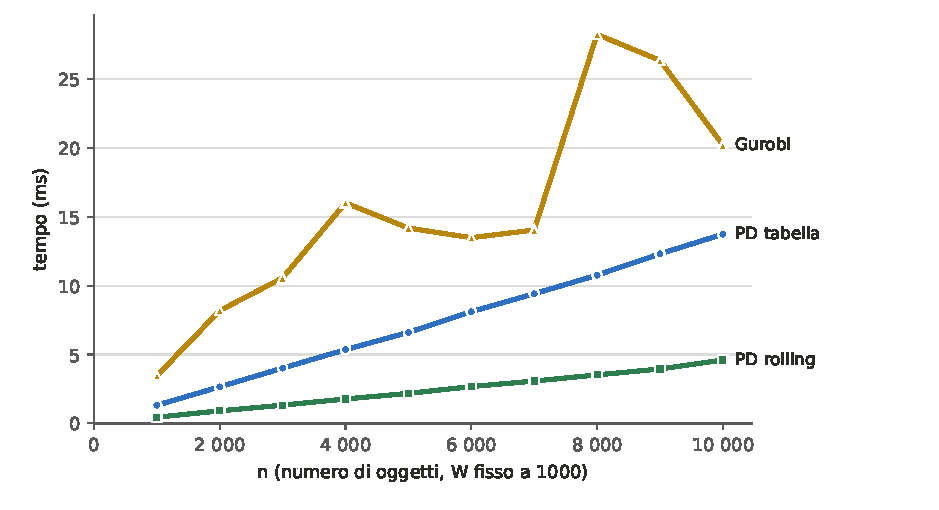
\includegraphics[width=0.82\linewidth]{../relazione/fig/tempo-vs-n.pdf}
  \end{center}
  {\small Lineare in $n$ a capacit\`a fissa ($R^2 = 0{,}9996$). Gurobi, usato come
  riscontro esterno, oscilla senza un andamento riconoscibile.}
\end{frame}

% ---------------------------------------------------------
\begin{frame}{\dots e cresce anche con la capacit\`a}
  \begin{center}
    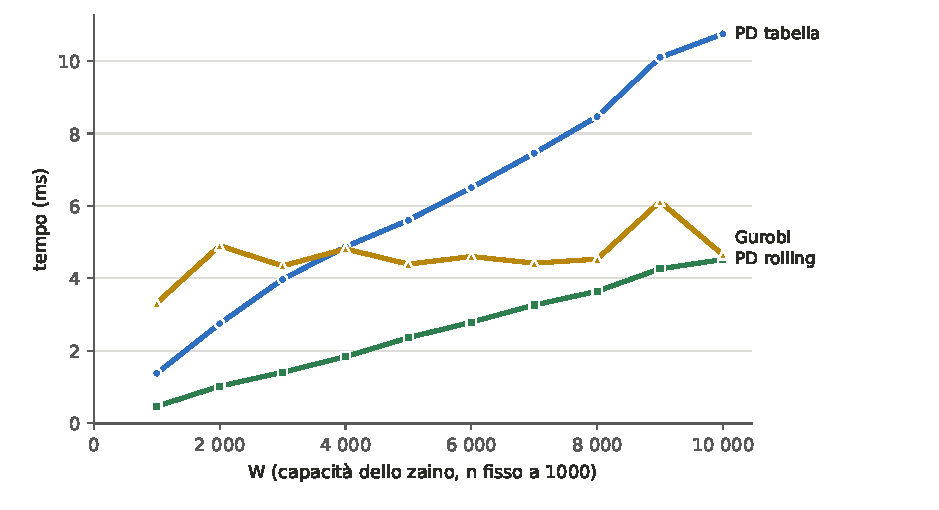
\includegraphics[width=0.82\linewidth]{../relazione/fig/tempo-vs-W.pdf}
  \end{center}
  {\small Qui il solver resta piatto: per lui $W$ \`e un coefficiente, per la
  programmazione dinamica una dimensione della tabella. \`E la
  pseudo-polinomialit\`a vista dal vivo.}
\end{frame}

% ---------------------------------------------------------
\begin{frame}{La memoria segue la formula}
  \begin{center}
    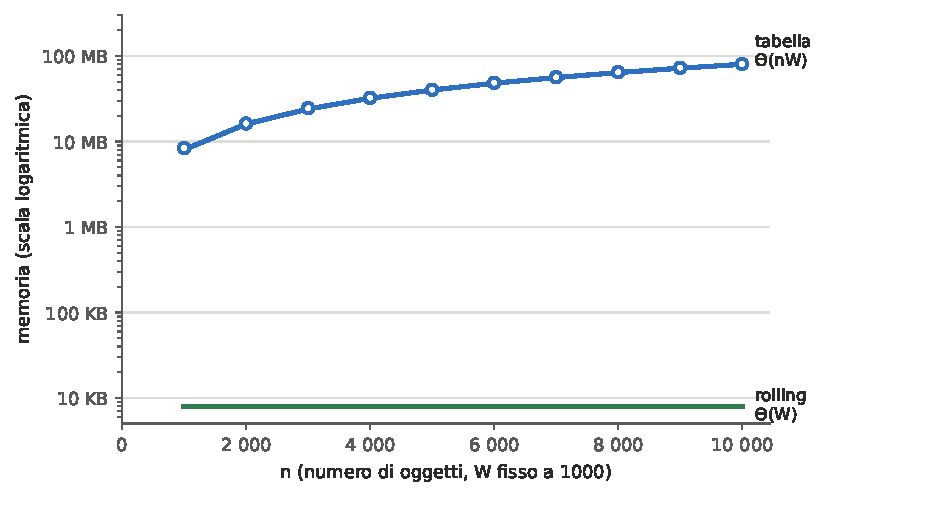
\includegraphics[width=0.78\linewidth]{../relazione/fig/memoria.pdf}
  \end{center}
  {\small Misura sull'heap entro il 5\% da $(n+1)(W+1)\cdot 8$ byte. Il rolling
  array sta quattro ordini di grandezza pi\`u in basso.}
\end{frame}

% ---------------------------------------------------------
\begin{frame}{Il limite pratico}
  Con $n = 2000$ e heap da 2 GB, al crescere della sola capacit\`a:
  \vfill
  \begin{center}
  \begin{tabular}{rrlrl}
    \toprule
    $W$ & \multicolumn{2}{c}{tabella $\To(nW)$} & \multicolumn{2}{c}{rolling $\To(W)$} \\
    \midrule
    $100\,000$    & 1,5 GB  & 0,76 s           & 781 KB & 0,09 s \\
    $300\,000$    & 4,5 GB  & memoria esaurita & 2,3 MB & 0,27 s \\
    $1\,000\,000$ & 14,9 GB & memoria esaurita & 7,6 MB & 0,92 s \\
    \bottomrule
  \end{tabular}
  \end{center}
  \vfill
  A parit\`a di tempo asintotico, la riduzione dello spazio estende di oltre un
  ordine di grandezza le istanze trattabili.
\end{frame}

% ---------------------------------------------------------
\begin{frame}{In sintesi}
  \begin{itemize}
    \item Entrambi i criteri di applicabilit\`a sono verificati, e la ricorrenza
          si traduce in due algoritmi: valore e ricostruzione.
    \item L'analisi prevede il comportamento osservato con precisione: tempo
          lineare in ciascun fattore, memoria entro il 5\% dalla formula.
    \item Il limite si presenta prima sulla memoria che sul tempo: da qui
          l'utilit\`a della variante a spazio ridotto.
    \item Correttezza verificata da 305 test e da un solver ILP usato come
          oracolo esterno.
  \end{itemize}
  \vfill
  \centering{\small Segue una breve demo: tabella $K$ ispezionabile,
  ricostruzione della soluzione, confronto fra le varianti.}
\end{frame}

\end{document}
